\section{Le cadre de travail}


\subsection{Observatoire de Paris}

L’Observatoire de Paris est un Grand Établissement sous tutelle du ministère de l’Enseignement supérieur et de la Recherche. Il a le statut d’EPSCP (Établissement public à caractère scientifique, culturel et professionnel). Ses trois missions principales sont : 1) la recherche, en contribuant au progrès de la connaissance de l’Univers par l’acquisition de données d’observation, le développement et l’exploitation des moyens appropriés, l’élaboration des outils théoriques nécessaires, 2) la formation initiale et continue, 3) la diffusion des connaissances. L’Observatoire de Paris abrite l’École Doctorale Astronomie et Astrophysique d’Île-de-France.

L’Observatoire de Paris compte un grand total d'environ 600 emplois permanents. Du coté MESR - 89 CNAP, 10 EC, 2 PRAG et 232 personnels de soutien; 248 titulaires du CNRS y sont affectés. L’Observatoire a le statut d'université et dispense un enseignement universitaire de haut niveau en astronomie et astrophysique allant du master au doctorat, avec possibilité de formation à distance, 245 étudiants y sont inscrits (ce chiffre intègre les étudiants des universités partenaires); par ailleurs 35 enseignants-chercheurs d’autres établissements de l’enseignement supérieur et 9 personnels divers travaillent dans les laboratoires de l’établissement; l’établissement emploie 42 contractuels dont 11 sur postes vacants, 19 sur contrat CNRS, le reste sur budget de l’établissement; son budget annuel hors salaires est de 20 M\euro\ et sa masse salariale est estimée à 35 M\euro.

\begin{figure}[!ht]
    \centerline{
    	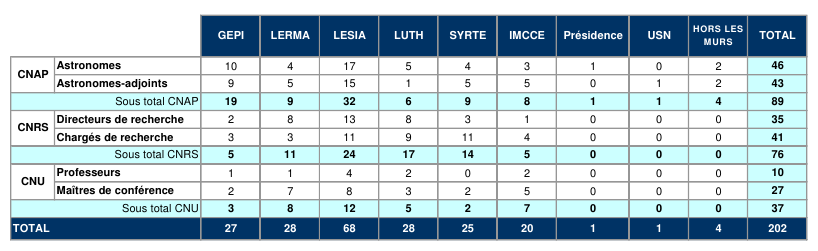
\includegraphics[width=1.3\textwidth]{./images/repartition_effectif.png}
    	}
    \caption{Répartition des effectifs (chercheurs et EC) par composante et par corps}
	%\centerline{}
		%\centerline{Source - Bilan Sociale 2010 http://ca.obspm.fr/IMG/pdf/09_Bilan-social-2010.pdf}
    \label{repartition_effectif}
\end{figure}

Cette institution représente le plus grand pôle national de recherche en astronomie. Il a été fondé en 1667. Près d’un tiers (30 \%) des astronomes français y poursuivent leurs recherches au sein de sept laboratoires situés sur trois campus (Paris fondé en 1667 par Louis XIV, Meudon fondé en 1876 par Jules Janssen dans des bâtiments du château de Meudon et Nançay construit en 1953 sur un terrain de l’ENS).

Il existe un partenariat fort entre l’Observatoire et le CNRS/INSU car les laboratoires de recherches sont tous des “Unités mixtes de recherche” et, souvent, en rattachement secondaire à d’autres universités scientifiques.

Les activités de recherche de l’Observatoire de Paris sont structurées autour de:


\begin{itemize}
\item[$\bullet$] 5 UMR associées au CNRS:
	\begin{itemize}
	\item GEPI: Galaxies, Étoiles, Physique et Instrumentation
	\item LERMA: Laboratoire d’Études du Rayonnement et de la Matière en Astrophysique
	\item LESIA: Laboratoire d’Études Spatiales et d’Instrumentation en Astrophysique
	\item LUTH: Laboratoire Univers et Théories
	\item SYRTE: SYstèmes de Référence Temps Espace
	\end{itemize}
\item[$\bullet$] 1 institut qui est aussi une UMR CNRS:
	\begin{itemize}
	\item IMCCE: Institut de mécanique céleste et de calcul des éphémérides
	\end{itemize}
\item[$\bullet$] 1 unité de service et de recherche:
	\begin{itemize}
	\item La station radioastronomique de Nançay
	\end{itemize}
\item[$\bullet$] 1 laboratoire de recherche associé ayant pour tutelle principale l’Université de Paris-Diderot, Paris 7:
	\begin{itemize}
	\item APC: AstroParticule et Cosmologie
	\end{itemize}
\item[$\bullet$] 1 unité mixte de service, créée en 2002, qui regroupe les services communs et centraux.
\item[$\bullet$] 1 unité de Formation et Enseignement\\
\end{itemize}

%\newline
\newpage
\subsection{Matériels utilisés}
J'ai utilisé divers ordinateurs, de l'ordinateur personnel (PC sous Linux) à des serveurs multi-cœurs avec des dizaines d'usagers, tout au laboratoire qu'à la DIO.

La DIO (Division Informatique de l’Observatoire) est un service chargé de tous les aspects informatiques mutualisés de l’Observatoire de Paris: système et réseau, calcul, stockage ainsi que du système d’information, de la bureautique des services centraux et de l’infrastructure technique de l’Observatoire virtuel.

Pour accéder aux services numérique gérés par la DIO un compte LDAP m'a été créé. Via ce compte je pouvais aussi accéder au courriel electronique (@obsmp.fr) et au réseau sans-fils interne. Ce compte LDAP permet aussi d'atteindre le réseau interne via un rebond SSH sur un des deux "firewall" (physiquement 1 à Meuden et 1 à Pais).\\

Le travail a été effectué sur une machine personnel, et des serveurs du LERMA et de la DIO:\\

\begin{itemize}
\item \textsc{\Large aramis}

	un serveur sous CentOS Linux version 5.9,\\
	avec 8 c\oe urs (deux Intel\textregistered\ Xeon\textregistered\ CPU           X5450  @ 3.00GHz)  64 bits\\
	et 16 Go de mémoire vive.
	\\
\item \textsc{\Large m2paris} (DIO UFE)

	un serveur sous Debian Linux version 7,\\
	avec 16 c\oe urs (deux Intel\textregistered\ Xeon\textregistered\ CPU           L5520  @ 2.27GHz)  64 bits\\
	et 12 Go de mémoire vive.
	\\
\item \textsc{\Large medusa}

	un serveur sous CentOS Linux version 5.9,\\
	avec 48 c\oe urs (quatre AMD Opteron\textregistered\  6176 SE @ 2.3GHz) 64 bits\\
	et 128 Go de mémoire vive.
	\\
\item \textsc{\Large haka}

	une machine personnelle sous Ubuntu Linux version 12.04.2,\\
	avec Intel\textregistered\ Core\textregistered 2 CPU          6400  @ 2.13GHz  32 bits\\
	et 2 Go de mémoire vive.
\end{itemize}



\begin{figure}
        \centering
        \begin{subfigure}[b]{0.5\textwidth}
                \centering
                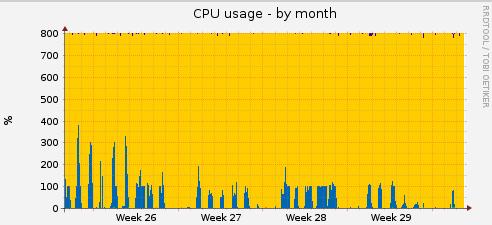
\includegraphics[width=\textwidth]{./images/aramis-cpu-monthm.png}
                \caption{\textsc{\large aramis}}
                %\centerline{Source - https://sionet.obspm.fr/munin/lerma-a111/aramis/cpu-month.png}
                \label{aramis}
        \end{subfigure}%
        ~
        \begin{subfigure}[b]{0.5\textwidth}
                \centering
                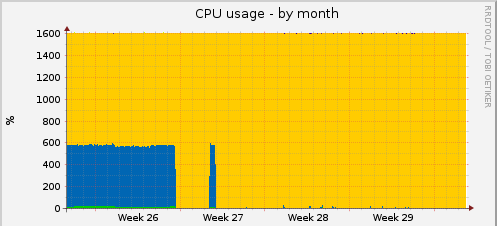
\includegraphics[width=\textwidth]{./images/m2paris-cpu-monthm.png}
                \caption{\textsc{\large m2paris}}
                %\centerline{Source - https://sionet.obspm.fr/munin/ufe/m2dsg-pro.obspm.fr/cpu-month.png}
                \label{m2paris}
        \end{subfigure}
        
        \begin{subfigure}[b]{0.5\textwidth}
                \centering
                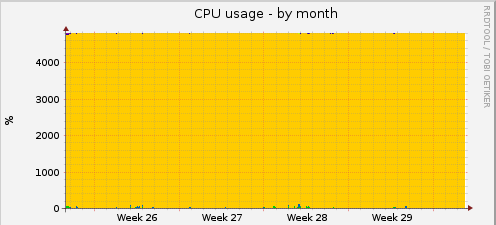
\includegraphics[width=\textwidth]{./images/medusa-cpu-monthm.png}
                \caption{\textsc{\large medusa}}
               %\centerline{Source -  https://sionet.obspm.fr/munin/lerma-b15/medusa/cpu-month.png}
                \label{medusa}
        \end{subfigure}
        \caption{La charge des serveurs pour le mois de juillet 2013 vu par l'outil Mumin}\label{charge_serveurs}
        \label{charge}
\end{figure}
\newpage
J'utilisais la machine personnelle (\textsc{\large haka}) pour connecter aux autres machines plus puissantes.
Compiler un projet, tel que GDL qui contient plus de 120 000 lignes de codes sur un machine comme \textsc{\large haka} va prendre environ 10 minutes, quand sur un serveur comme \textsc{\large aramis} la compilation va prendre au maximum 2 minutes quand la machine est partiellement chargée.

La charge des serveurs a été une des raisons d'avoir plusieurs machines à disposition, sur la Figure \ref{charge} on voit que la machine \textsc{\large aramis} est partiellement chargé (Figure \ref{aramis}), la machine \textsc{\large m2paris} est chargé de manière plus permanente (Figure \ref{m2paris}) et la charge de la machine \textsc{\large medusa} est négligeable (Figure \ref{medusa}). Le fait d'avoir à disposition des machines qui sont chargés a ses avantages, bien sur la majorité de travail est fait sur une machine avec la charge insignifiante pour diminuer le temps de compilation. Dès que la correction de code est terminé il faut tester le logiciel dans des environnements variés pour conforter son comportement. Notamment la dépendance aux versions de GCC et les problèmes liées aux architectures (32/64 bits). Dans un environnement chargé a été trouvé le problème avec les nombres des threads de OpenMP défini dans GDL (plus de détailles dans le section \ref{num_thread}, page \pageref{num_thread}). 

L'autre a été l'exigence de tester son compatibilité avec des systèmes d'exploitations et des architectures variées.

\subsection{Logiciels utilisés}
Les systèmes d'exploitation que j'ai utilisés pendant le stage étaient les différentes distributions de Linux et parfois Mac OS X. Pendent le stage je travaillais uniquement en mode commande. Les logiciels les plus utilisés sont cités ci-dessous:


\begin{description}
  \item[GNU Compiler Collection (GCC)] \hfill \\
	Crée en 1987 \textbf{GCC} est un ensemble de compilateurs portés sur les majorités de systèmes d'exploitation (Linux, Unix, Windows etc\ldots) et de microprocesseurs (x86, AMD64, ARM, SPARC etc\ldots). Il a été créé par le projet GNU comme un compilateur de langage C, mais après quelques années de développement il est devenu beaucoup plus fonctionnel que juste un compilateur.\\
	Aujourd'hui \textbf{GCC} est très extensible et adaptable aux besoins des utilisateurs, il contient aussi les compilateurs pour nombreux langages de programmation, tels que C, C++, Objective-C, Java, Ada, Fortran et d'autres langages, plus ou moins connus. \textbf{GCC} est le compilateur fourni avec nombreux systèmes d'exploitation comme Linux, BSD, Mac OS X ou BeOS. La plupart des logiciels libres sont compilée avec \textbf{GCC}, car en plus d’être performant, il est libre au sens de la licence GNU GPL.\\
	D’après tout ça on comprend pourquoi on a choisi \textbf{GCC} comme compilateur pour le projet GDL.
	\\ \\
  \item[GNU Debugger (GDB)] \hfill \\
  \textbf{GDB} a été créé en 1988  par Richard Stallman comme le débogueur standard du projet GNU. Comme pour  \textbf{GCC} il existe des ports de \textbf{GDB}  sur différent types de microprocesseurs et systèmes d'exploitation, il supporte différents langages de programmation et il est distribué sous les termes de la licence GNU GPL.\\
  \textbf{GDB} propose de nombreuses fonctionnalités pour tracer et contrôler l’exécution d'un programme informatique pas à pas. On peut surveiller ou modifier (si il y a besoin) une variable interne, on peut aussi faire un appel à fonction, indépendant du comportement prévu dans le programme. \textbf{GDB}  permet le débogage distant selon gdbserver, qui est lancé sur la même machine que le programme et le débogage est effectuer d'une autre. Cette technique est souvent utilisée pour déboguer un programme sur un système embarqué.
  \\ \\
  \item[Valgrind] \hfill \\
L'une des plus grandes difficultés de C++ est de gérer correctement la mémoire, alors pour diminuer les problèmes liés à la fuite de mémoire (l'absence de désallocation  de l'espace utilisé, double désallocation de l'espace utilisé etc\ldots) j'ai utilisé  \textbf{Valgrind}.\\
	A l'origine il a été crée comme un débogueur de mémoire pour Linux sur architecture x86, mais depuis il est devenue un plate-forme d'analyse dynamique pour les contrôleurs de la mémoire et "profilers". Il est disponible pour les systèmes d'exploitation Linux, Mac OS X et Android sur les microprocesseurs x86, x86-64, PowerPC et ARM. Grâce à sa licence GNU GPL v2,  il existe des ports non-officiels sur d'autres systèmes et architectures.\\
	Essentiellement \textbf{Valgrind} est un machine virtuelle utilisant la technique de compilation à la volée, le programme d'origine ne s’exécute pas directement sur un processeur, avant d’exécution il est traduit dans une représentation intermédiaire simplifié, les instructions sont ajoutées par un outil ("memcheck", "profiler" ou un outil externe) et finalement ces instructions sont traduites dans un code machine. A cause des procédures de traduction sous \textbf{Valgrind} l’exécution d'un programme est au moins 5 fois plus lent.\\
	Il est possible de combiner \textbf{Valgrind} avec \textbf{GDB} pour profiter des avantages de ces deux excellents outils.
\end{description}


\begin{figure}
        \centering
        \begin{subfigure}[b]{0.3\textwidth}
                \centering
    			
\includegraphics[width=0.4\textwidth]{./images/gcc.png}
                \caption{\textsc{GCC}}
				%\centerline{Source - http://upload.wikimedia.org/wikipedia/commons/thumb/a/a9/	Gccegg.svg/500px- Gccegg.svg.png}
                \label{logo-gcc}
        \end{subfigure}%
        ~
        \begin{subfigure}[b]{0.3\textwidth}
                \centering
                
\includegraphics[width=0.5\textwidth]{./images/gdb.png}
                \caption{\textsc{GDB}}
                %\centerline{Source - https://upload.wikimedia.org/wikipedia/commons/6/6a/Archer.jpg}
                \label{logo-gdb}
        \end{subfigure}%
        ~
        \begin{subfigure}[b]{0.3\textwidth}
                \centering
                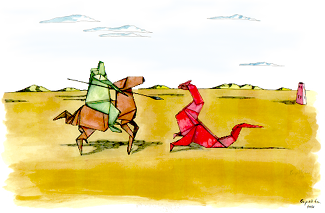
\includegraphics[width=0.7\textwidth]{./images/Valgrind_logo.png}
                \caption{\textsc{Valgrind}}
               %\centerline{Source -  https://upload.wikimedia.org/wikipedia/fr/f/f9/Valgrind_logo.png}
                \label{logo-valgrind}
        \end{subfigure}
        \caption{Les logos}\label{logos}
\end{figure}


